\documentclass{article}
 
%encoding
%--------------------------------------
\usepackage[utf8]{inputenc}
\usepackage[T1]{fontenc}
%--------------------------------------

%Trigonometric Circle
%--------------------------------------
\usepackage{tikz}
\usetikzlibrary{datavisualization.formats.functions,backgrounds,calc,angles}
\def\mytypesetter#1{% page 813
  \pgfmathparse{#1/pi}%
  \pgfmathprintnumber{\pgfmathresult}$\pi$%
}
%--------------------------------------

\usepackage[landscape]{geometry}
\usepackage{url}
\usepackage{multicol}
\usepackage{amsmath}
\usepackage{amsfonts}
\usepackage{tikz}
\usepackage{amsmath,amssymb}
\usepackage{ragged2e}

\usepackage{colortbl}
\usepackage{xcolor}
\usepackage{mathtools}
\usepackage{amsmath,amssymb}
\usepackage{enumitem}
\makeatletter

\newcommand*\bigcdot{\mathpalette\bigcdot@{.5}}
\newcommand*\bigcdot@[2]{\mathbin{\vcenter{\hbox{\scalebox{#2}{$\m@th#1\bullet$}}}}}
\makeatother

\title{PHY335 - Examen 1}
\author{Sophie Bernadin-Mercier}

\advance\topmargin-.8in
\advance\textheight3in
\advance\textwidth3in
\advance\oddsidemargin-1.5in
\advance\evensidemargin-1.5in
\parindent0pt
\parskip2pt
\newcommand{\hr}{\centerline{\rule{3.5in}{1pt}}}
\begin{document}

\begin{center}
{\large{\textbf{PHY335 - Examen 1}}}\\
{\small Hivers 2020 | Sophie Bernadin-Mercier}\\
{\small \textcolor{blue}{github.com/Shuhala/latExTS}}
\end{center}

\begin{multicols*}{3}

\tikzstyle{mybox} = [draw=black, fill=white, thick,
    rectangle, rounded corners, inner sep=10pt, inner ysep=10pt]
\tikzstyle{fancytitle} =[fill=white, text=black, font=\bfseries]

%------------ Equation de deplacement ---------------------
\begin{tikzpicture}
\node [mybox] (box){%
    \begin{minipage}{0.3\textwidth}
    $$x(t)= A cos(\omega t + \varphi)$$
    $$v(t)= - \omega A sin(\omega t + \varphi)$$

    $\begin{array}{l}
    x_1=A cos \alpha _1 \\
    v_1=- \omega A sin \\
    \alpha _1 = \omega t_1 + \varphi
    \end{array}$ donc 
    $\begin{cases}
    A^2 = x_1^2 + (\frac{v_1}{\omega})^2 \\
    tan\;\alpha _1 = \frac{-v_1}{\omega x_1}
    \end{cases}$
    \end{minipage}
};
\node[fancytitle, right=10pt] at (box.north west) {Equation de deplacement};
\end{tikzpicture}

%------------ Position d'equilibre ---------------------
\begin{tikzpicture}
\node [mybox] (box){%
    \begin{minipage}{0.3\textwidth}
        
    $PE = l_0 + \Delta l$ \\
    $x_0 = x - PE \textcolor{red}{*}$
    
    \scriptsize{Pour les systemes en angle (gauche a droite ou droite a gauche), la position d'equilibre sera calcule (j'pense) kind of comme ci-dessous.}
        
    \begin{multicols}{2}
        \begin{minipage}{.15\textwidth}
            \begin{tikzpicture}[scale=0.3]
                \draw[->,font=\tiny] (1,0) -- (0,1) node[above left=-0.8em] {x};
                \draw[<-,font=\tiny] (1.5,0) node[below right=-0.8em] {v} -- (0.5,1);
            \end{tikzpicture}
        \end{minipage}%
        \begin{minipage}{.15\textwidth}
        $l_0 + \Delta l$
        \end{minipage}
        
        \begin{minipage}{.15\textwidth}
            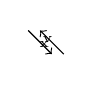
\begin{tikzpicture}[scale=0.3]
                \draw[<-,font=\tiny] (1,0) node[below right=-0.8em] {x} -- (0,1);
                \draw[->,font=\tiny] (1.5,0) -- (0.5,1) node[above left=-0.8em] {v};
            \end{tikzpicture}
        \end{minipage}%
        \begin{minipage}{.15\textwidth}
        $l_0 - \Delta l$
        \end{minipage}
        \end{multicols}
        
        \begin{multicols}{2}
        \begin{minipage}[t]{.15\textwidth}
            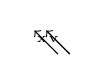
\begin{tikzpicture}[scale=0.3]
                \draw[->,font=\tiny] (1,0) -- (0,1) node[above left=-0.8em] {x};
                \draw[->,font=\tiny] (1.5,0) -- (0.5,1) node[above left=-0.8em] {v};
            \end{tikzpicture}
        \end{minipage}%
        \begin{minipage}[t]{.15\textwidth}
        $l_0 - \Delta l$
        \end{minipage}
        
        \begin{minipage}{.15\textwidth}
            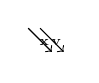
\begin{tikzpicture}[scale=0.3]
                \draw[<-,font=\tiny] (1,0) node[below right=-0.8em] {x} -- (0,1);
                \draw[<-,font=\tiny] (1.5,0) node[below right=-0.8em] {v} -- (0.5,1);
            \end{tikzpicture}
        \end{minipage}%
        \begin{minipage}{.15\textwidth}
        $l_0 + \Delta l$
        \end{minipage}
        \end{multicols}
    
    \scriptsize{\textcolor{red}{*} Si compresse et direction oppose a l'axe des x: $x_0 = PE - x$}
    
    \end{minipage}
};
\node[fancytitle, right=10pt] at (box.north west) {Position d'equilibre};
\end{tikzpicture}

%------------ Variables ---------------
\begin{tikzpicture}
\node [mybox] (box){%
    \begin{minipage}{0.3\textwidth}
    \small{
    	\begin{tabular}{>{\raggedleft\arraybackslash}p{4.2cm}>{\raggedright\arraybackslash}p{3.3cm}}
		\textit Amplitude (A) &
		    $=\sqrt{x_0^2+(\frac{v_0}{\omega})^2}$ \\
		    \noalign{\vskip 3pt}
		    \hline
		    \noalign{\vskip 3pt}
		\textit Phase initiale de l'origine ($\varphi$) & 
		    $\omega t_0 + \varphi= tan^{-1}(- \frac{v_0}{\omega x_0})$ \\
		    \noalign{\vskip 3pt}
		    \hline
		    \noalign{\vskip 3pt}
		\textit Energie potentielle (U) & 
		    $=\frac{1}{2}kx^2$ \\
		    \noalign{\vskip 3pt}
		    \noalign{\vskip 3pt}
	    \textit Systeme oscillant a la verticale & 
		    $U=U_R + U_G J\newline
		    U_R=\frac{1}{2}k \Delta l^2 J\newline
		    U_g=m g h$ J\\
		    \noalign{\vskip 3pt}
		    \hline
		    \noalign{\vskip 3pt}
		\textit Energie cinetique (K) & 
		    $=\frac{1}{2} m v^2$ J\\
		    \noalign{\vskip 3pt}
		    \hline
		    \noalign{\vskip 3pt}
		\textit Energie total (E) & 
		    $=U+K=\frac{1}{2}kA^2$ J\\
		    \noalign{\vskip 3pt}
		    \hline
		    \noalign{\vskip 3pt}
	    \textit Frequence angulaire ($\omega$) pulsation & 
		    $=2 \pi f = \sqrt{\frac{k}{m}} = \sqrt{\frac{g}{l}} $ \\
            \noalign{\vskip 3pt}
		    \hline
		    \noalign{\vskip 3pt}
	    \textit Periode (T) & 
		    $=\frac{2\pi}{\omega}=\frac{1}{f}$ \\
		    \noalign{\vskip 3pt}
		    \hline
		    \noalign{\vskip 3pt}
	     \textit Elongation maximale ($\Delta l_{max}$) & 
		    $= \Delta l \cdot 2$ \\
		    \noalign{\vskip 3pt}
		    \hline
		    \noalign{\vskip 3pt}
	     \textit Elongation ($\Delta l$) & 
		    $= \frac{m \cdot g \cdot sin\theta}{k}$ \\
		    \noalign{\vskip 3pt}
		    \hline
		    \noalign{\vskip 3pt}
	    \textit Dephasage ($\Delta \alpha$) & 
		    $\alpha _A = \omega t_0 + \varphi \newline
		    \alpha _B = \omega (t_0 + \Delta t) + \varphi \newline
		    \Delta \alpha = \alpha _B - \alpha _A = \omega \Delta t$ \\
	\end{tabular}}
    \end{minipage}
};
\end{tikzpicture}

\vfill\columnbreak

%------------ Expression des MHS ---------------
\begin{tikzpicture}
\node [mybox] (box){%
    \begin{minipage}{0.3\textwidth}
    	$x_n=A_n cos(\omega t + \varphi _n)$ \\ \\
        $a=A_1 cos\varphi _1 + A_2 cos\varphi _2 + ... + A_n cos\varphi _n $ \\
        $b=A_1 sin\varphi _1 + A_2 sin\varphi _2 + ... + A_n sin\varphi _n $ \\ \\
        $A_R=\sqrt{a^2+b^2}$ \\
        $\psi _R=tan^{-1}(\frac{b}{a})$ \\ \\
        $x_R(t)=A_R \cdot cos(\omega \cdot t + \psi _R)$
    \end{minipage}
};
\node[fancytitle, right=10pt] at (box.north west) {Expression des MHS};
\end{tikzpicture}

%------------ Equation de la trajectoire ---------------
\begin{tikzpicture}
\node [mybox] (box){%
    \begin{minipage}{0.3\textwidth}
        $$(\frac{x}{A_x})^2 + (\frac{y}{A_y})^2 - \frac{2 x y}{A_x A_y} \; cos(\Delta \varphi )=sin^2(\Delta \varphi)$$
    \end{minipage}
};
\node[fancytitle, right=10pt] at (box.north west) {Equation de la trajectoire};
\end{tikzpicture}

%------------ Variables ---------------
\begin{tikzpicture}
\node [mybox] (box){%
    \begin{minipage}{0.3\textwidth}
    \small{
    	\begin{tabular}{>{\raggedleft\arraybackslash}p{5cm}>{\raggedright\arraybackslash}p{2cm}}
        \textit Frequence (f) & 
		    $=\frac{1}{T} Hz$ \\
		    \noalign{\vskip 3pt}
		    \hline
		    \noalign{\vskip 3pt}
		 \textit Periode d'oscillation ($T_{osc}$) &
		    $=\frac{1}{f_{osc}}$ \\
		    \noalign{\vskip 3pt}
		    \hline
		    \noalign{\vskip 3pt}
	     \textit Courbe AR(t) oscille à la frequence ($f_{A_R}$) &
		    $=\frac{f_2 - f_1}{2}\;Hz$ \\
		    \noalign{\vskip 3pt}
		    \hline
		    \noalign{\vskip 3pt}
	     \textit Frequence de battement ($f_b$) &
		    $= | f_2 - f_1 |\;Hz$ \\
		    \noalign{\vskip 3pt}
		    \hline
		    \noalign{\vskip 3pt}
	     \textit Moyenne de frequence ($f_{moy}$) &
		    $=\frac{f_1 + f_2}{2}\;Hz$ \\
	\end{tabular}}
    \end{minipage}
};
\end{tikzpicture}

%------ oscillations harmoniques------
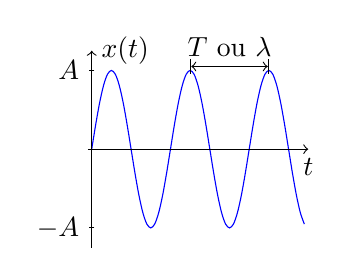
\begin{tikzpicture}[scale=0.5]
	\def \xLabel {$t$}; % legende sur x
    \def \yLabel {$x(t)$}; % legende sur y
    \def \xmin{-0.1}; 
    \def \xmax{5.5};
    \def \ymin{-2.5};
    \def \ymax{2.5};
    \draw[smooth,color=blue, variable=\x, samples at={0,0.1,...,5.5}]   plot (\x,{2*sin(\x r*pi)}) ;
    \draw[->] (\xmin,0) -- (\xmax,0) node[below] {\xLabel};
    \draw[->] (0,\ymin) -- (0,\ymax) node[right] {\yLabel};
    \foreach \y/\ytext in {-2/-A,2/A} 
    \draw[shift={(0,\y)}] (2pt,0pt) -- (-2pt,0pt) node[left] {$\ytext$};  
    \draw[|<->|] (2.5,2.1)--++(2,0) node[pos=0.5, above]{$T$ ou $\lambda$};
\end{tikzpicture}

%------------ Trigonometric circle ---------------
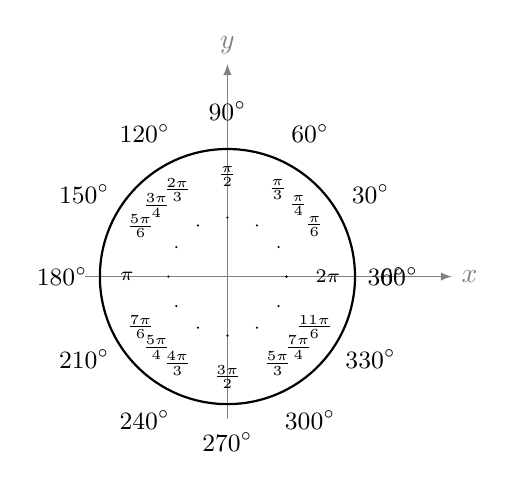
\begin{tikzpicture}[scale=1.5,cap=round,>=latex,baseline={(0,0)}]
    %/ Axes
    \draw[->,gray] (-1.2cm,0cm) -- (1.9cm,0cm) node[right,fill=white] {$x$};
    \draw[->,gray] (0cm,-1.2cm) -- (0cm,1.8cm) node[above,fill=white] {$y$};
    
    %/ Circle
    \draw[thick] (0cm,0cm) circle(1.08cm);
    
    \foreach \x in {0,30,...,360} {
        % lines from center to point
        %\draw[gray] (0cm,0cm) -- (\x:1cm);
        % dots at each point
        \filldraw[black] (\x:0.5cm) circle(0.1pt);
        % draw each angle in degrees
        \draw (\x:1.4cm) node {\small{$\x^\circ$}};
    }
    
    %/ Radian
    \foreach \x/\xtext in {
      30/\frac{\pi}{6},
      45/\frac{\pi}{4},
      60/\frac{\pi}{3},
      90/\frac{\pi}{2},
      120/\frac{2\pi}{3},
      135/\frac{3\pi}{4},
      150/\frac{5\pi}{6},
      180/\pi,
      210/\frac{7\pi}{6},
      225/\frac{5\pi}{4},
      240/\frac{4\pi}{3},
      270/\frac{3\pi}{2},
      300/\frac{5\pi}{3},
      315/\frac{7\pi}{4},
      330/\frac{11\pi}{6},
      360/2\pi}
    \draw (\x:0.85cm) node {\scriptsize{$\xtext$}};
\end{tikzpicture}

\vfill\columnbreak

%------------ Equation de l'onde ---------------
\begin{tikzpicture}
\node [mybox] (box){%
    \begin{minipage}{0.3\textwidth}
            $y(x,t)=A cos(\omega t \pm kx+\varphi)\;cm$ \\\\
            $y_i = A cos (\omega t - k x)$ \\
            $y_r = A cos (\omega t - k x)$ \\
            $y(x,t) = 2 A cos(k x) cos(\omega )$ \\\\
            \scriptsize{
                Ondes se propageant en direction de \\
                \textbf{x > 0: }
                $(\omega t - k x)$ et $(k x - \omega t)$ \\
                \textbf{x < 0: }
                $(\omega t + k x)$ et $(- \omega t - k x)$
            }
        
    \end{minipage}
};
\node[fancytitle, right=10pt] at (box.north west) {Equation de l'onde};
\end{tikzpicture}

%------------ Variables ---------------
\begin{tikzpicture}
\node [mybox] (box){%
    \begin{minipage}{0.3\textwidth}
    \small{
    	\begin{tabular}{>{\raggedleft\arraybackslash}p{4cm}>{\raggedright\arraybackslash}p{3.5cm}}
		 \textit Phase de l'onde &
		    $(\omega t \pm kx + \varphi)$ \\
		    \noalign{\vskip 3pt}
		    \hline
		    \noalign{\vskip 3pt}
	     \textit Nombre d'onde (k) $m^{-1}$ &
		    $=\frac{\omega}{c}=\frac{2\pi}{\lambda}$ \\
		    \noalign{\vskip 3pt}
		    \hline
		    \noalign{\vskip 3pt}
	     \textit Longueur d'onde ($\lambda$) &
		    $=c T=\frac{c}{f}$ \\
		    \noalign{\vskip 3pt}
		    \hline
		    \noalign{\vskip 3pt}
	     \textit Vitesse de propagation (c) &
		    $=\lambda f = \frac{\omega}{k} = \sqrt{\frac{F}{\mu}}$ \\
		    \noalign{\vskip 3pt}
		    \hline
		    \noalign{\vskip 3pt}
	     \textit Vitesse transversale ($v_y(x,t)$) cm/s &
	        $=\frac{\mathrm{d} }{\mathrm{d} t} y(x,t) \newline
	        =-A \omega sin(\omega t - k x + \varphi)$
		     \\
		    \noalign{\vskip 3pt}
		    \hline
		    \noalign{\vskip 3pt}
	     \textit Acceleration transversale ($a_y(x,t)$) cm/$s^2$ &
		    $=\frac{\mathrm{d} }{\mathrm{d} t} v_y(x,t) \newline
		    = -A \omega ^2 cos(\omega t - k x + \varphi) \newline
		    = - \omega ^2 y(x,t)$ \\
		    \noalign{\vskip 3pt}
		    \hline
		    \noalign{\vskip 3pt}
		 \textit Position max ($x_{max}$) &
		    $=A$ \\
		    \noalign{\vskip 3pt}
		    \hline
		    \noalign{\vskip 3pt}
	     \textit Vitesse max ($v_{max}$) &
		    $=\omega A$ \\
		    \noalign{\vskip 3pt}
		    \hline
		    \noalign{\vskip 3pt}
	     \textit Acceleration max ($a_{max}$) &
		    $=\omega ^2 A$ \\
		    \noalign{\vskip 3pt}
		    \hline
		    \noalign{\vskip 3pt}
	     \textit Impedance de la corde Z kg/s &
		    $=\frac{F_y}{v}=\frac{F k}{\omega}=\frac{F}{c}=\mu c \newline = \sqrt{\mu F}$ \\
		    \noalign{\vskip 3pt}
		    \hline
		    \noalign{\vskip 3pt}
	     \textit Puissance instantanee $\Bar{W}$ &
		    $=\frac{Z \omega ^2 A^2}{2}$ \\
		    \noalign{\vskip 3pt}
		    \hline
		    \noalign{\vskip 3pt}
	     \textit Puissance transportee par l'onde progressive & 
	        $W(x,t)=Z \omega ^2 A^2 sin^2(\omega t - k x + \varphi)$ \newline 
	        $W(x_0,t)=Z \omega ^2 A^2 sin^2 (\omega t + \varphi )$ \\
		    \noalign{\vskip 3pt}
		    \hline
		    \noalign{\vskip 3pt}
	     \textit Coefficient de reflexion en puissance ($R$) &
		    $=\frac{\bar{W_r}}{\bar{W_i}} =(\frac{A_r}{A_i})^2
		    \newline =(\frac{Z_1-Z_2}{Z_1+Z_2})^2=r^2$ \\
		    \noalign{\vskip 3pt}
		    \hline
		    \noalign{\vskip 3pt}
	     \textit Coefficient de transmission en puissance ($T$) &
		    $=\frac{\bar{W_t}}{\bar{W_i}} =\frac{Z_2}{Z_1} (\frac{A_t}{A_i})^2
		    \newline = \frac{4 Z_1 Z_2}{(Z_1+Z_2)^2} = \frac{Z_2}{Z_1}\cdot t^2$ \\
	    \textit Puissance moyenne transportee par les 3 ondes &
		    $\bar{W_i}=\frac{Z_1 \omega ^2 A_i^2}{2}$ \newline
		    $\bar{W_r}=\frac{Z_1 \omega ^2 A_r^2}{2}$ \newline
		    $\bar{W_t}=\frac{Z_2 \omega ^2 A_t^2}{2}$ \\
	\end{tabular}}
	\scriptsize{
            Notes: \\
            - F est la mesure de cohésion élastique (tension N) \\
            - $\mu$ est la mesure d'inertie (g/m)
        }
    \end{minipage}
};
\end{tikzpicture}
\end{multicols*}
\newpage

%-----------------------
%---------------- PAGE 2
%-----------------------

\begin{multicols*}{2}

\tikzstyle{mybox} = [draw=black, fill=white, thick,
    rectangle, rounded corners, inner sep=10pt, inner ysep=10pt]
\tikzstyle{fancytitle} =[fill=white, text=black, font=\bfseries]

\begin{tikzpicture}
\node [mybox] (box){%
    \begin{minipage}{0.45\textwidth}
        \begin{tikzpicture}[scale=0.4]
    	\def \xLabel {$x$};
        \def \yLabel {$y$};
        \draw (0,2) coordinate[label=above right:$30^\circ$] (A) - - (0,0) coordinate (B) 
    - - (2,4) coordinate[label=above right:{$MHS_3 (1,\frac{\pi}{4})$}] (C) pic [draw] {angle= C--B--A};
        \draw (2,0) coordinate[label=above right:$45^\circ$] (A) - - (0,0) coordinate (B)
    - - (4,2) coordinate[label=above right:{$MHS_2 (2,\frac{\pi}{3})$}] (C) pic [draw] {angle};
        \draw[-] (0,0) -- (5,0) node[right] {$MHS_1 (3,\frac{\pi}{2})$};
        \draw[-] (0,5) node[above] {$MHS_4 (2,0)$} -- (0,0);
        \draw[->] (0,0) -- (5,0) node[below] {\xLabel};
        \draw[->] (0,0) -- (0,5) node[below left] {\yLabel};
        \end{tikzpicture}
        
        \centering
        \textbf{Selon x} \\
        $a_x = \underset{MHS_1}{3 cos(\frac{\pi}{2})} + cos(45^\circ) \cdot \underset{MHS_2}{2cos(\frac{\pi}{3})} + sin(30^\circ) \cdot \underset{MHS_3}{1 cos(\frac{\pi}{4})}=1.06$ \\
        $b_x = \underset{MHS_1}{3 sin(\frac{\pi}{2})} + cos(45^\circ) \cdot \underset{MHS_2}{2sin(\frac{\pi}{3})} + sin(30^\circ) \cdot \underset{MHS_3}{1 sin(\frac{\pi}{4})}=4.58$ \\
        \vskip 5pt
        $A_{R_x} = \sqrt{1.06^2 + 4.58^2}=4.6996$ \\
        $\psi_{R_x} = tan^{-1}(\frac{4.58}{1.06})=1.343$ \\
        \vskip 5pt
        $X_R(t) = 4.7 cos(\omega t + 1.3)$ \\
        \vskip 10pt
        \textbf{Selon y} \\
        $a_y = \underset{MHS_4}{2 cos(0)} + sin(45^\circ) \cdot \underset{MHS_2}{2cos(\frac{\pi}{3})} + cos(30^\circ) \cdot \underset{MHS_3}{1 cos(\frac{\pi}{4})}=3.32$ \\
        \vskip 5pt
        $b_y = \underset{MHS_4}{2 sin(0)} + sin(45^\circ) \cdot \underset{MHS_2}{2sin(\frac{\pi}{3})} + cos(30^\circ) \cdot \underset{MHS_3}{1 sin(\frac{\pi}{4})}=1.84$ \\
        \vskip 5pt
        $A_{R_y} = \sqrt{1.06^2 + 4.58^2}=3.79$ \\
        $\psi_{R_y} = tan^{-1}(\frac{4.58}{1.06})=0.51$ \\
        \vskip 5pt
        $Y_R(t) = 3.79 cos(\omega t + 0.51)$
        \vskip 10pt
        \textbf{Equation de la trajectoire} \\
        \vskip 5pt
        $(\frac{x}{4.7})^2 + (\frac{y}{3.79})^2 - \frac{2 x y}{4.7 \cdot 3.79} \; cos(0.51 - 1.3 )=sin^2(0.51 - 1.3)$
        \vskip 5pt
        $0.045 x^2 + 0.07 y^2 - 0.079 xy = 0.5046$
        
    \end{minipage}
};
\node[fancytitle, right=10pt] at (box.north west) {Exemple: Expression des MHS};
\end{tikzpicture}

%------------ Varia ---------------
\begin{tikzpicture}
\node [mybox] (box){
    \begin{minipage}{0.45\textwidth}
    1 rad = 0.1591549431 circle,\qquad 1 circle = 6.2831853072 rad \\\\
    $sin(1)=cos(1-\frac{\pi}{2})$,\qquad$cos(1)=sin(1+\frac{\pi}{2})$\\\\
    $sin=\frac{o}{h}$,\quad$cos=\frac{a}{h}$,\quad$tan=\frac{o}{a}$
    \end{minipage}
};
\node[fancytitle, right=10pt] at (box.north west) {Varia};
\end{tikzpicture}

\columnbreak

%------------ Exemple: Graphique d'onde ---------------
\begin{tikzpicture}
\node [mybox] (box){
    \begin{minipage}{0.45\textwidth}
    \textit{Onde sinusoidale se propage vers la gauche le long d'une corde de masse lineique de 25 g/m et soumise a une tension de 3.6 N. Figure inexistante illustre la corde a t=0. La fonction commence a 3.54 sur l'axe des y. L'echelle de la figure est: selon x, 1cm = 10cm et selon y, 1cm = 2mm} \\
    a) Amplitude: 5mm \\
    b) Longueur d'onde: $\lambda$ = 40cm \\
    c) Vitesse de propagation: $c=\frac{3.6N}{25/(1 \cdot 100 \cdot 10)}=12m/s=1200cm/s$ \\
    d) Frequence: $solve(1200=40 \cdot f,f)=30Hz$ \\
    e) Fonction d'onde: $y(x,t)=5cos(60\pi t + \frac{\pi}{20} x + \varphi)$\\
    $\omega=3 \pi f = 60\pi$,\qquad $k=\omega / c = \pi / 20$ \\
    $solve(y(0,0)=3.54, \varphi)=0.78\;ou\;5.5=0.78$ \\
    $y(x,t)=5cos(60\pi t + \frac{\pi}{20} x + 0.78)$ \\
    f) Vitesse maximale: $v_{max}=\omega A=60\pi 5 = 300 \pi$
    \end{minipage}
};
\node[fancytitle, right=10pt] at (box.north west) {Exemple: Graphique d'onde};
\end{tikzpicture}

%------------ Exemple: Plein d'ondes ---------------
\begin{tikzpicture}
\node [mybox] (box){
    \begin{minipage}{0.45\textwidth}
    \textit{On observe que 64\% de la puissance transportée par une onde incidente est transmise au second milieu. Cette corde, de masse linéique 1,5 g/cm est plus massive que la corde 1. Par ailleurs la tension est de 135N.} \\
    On deduit que \qquad $\mu _2 = 1.5 g/cm$,\qquad $F=135N$,\qquad $T=64\%$\\\\
    a) Impedances des deux milieux?
    $$Z_2 = \sqrt{1.5 \frac{\_gm}{\_cm} \cdot 135} = 4,5 kg/s$$
    $$solve(0.64=\frac{4 \cdot Z_1 \cdot 4.5}{(Z_1 + 4.5)^2}, Z_1) = 1,125\;or\;18=1,125 ??$$
    b) On sait que l'onde transmise transporte en moyenne 127.91 W et est caracterisee par une longueur d'onde de 1m et une phase initiale a l'origine de $-\frac{\pi}{2}$. Fonctions d'onde des trois ondes?
    $$T=\frac{\bar{W_T}}{\bar{W_i}}=0.64$$
    $$solve(\frac{127.91}{W_i}=0.64, W_i)=199,86 W$$
    $$W_i=\frac{Z_1 \omega^2 A_i ^2}{2}\;=\;...\tiny{Bed time}$$
    \end{minipage}
};
\node[fancytitle, right=10pt] at (box.north west) {Exemple: Plein d'ondes};
\end{tikzpicture}

%------------ End ---------------------
\end{multicols*}
\end{document}